%-*- coding: UTF-8 -*-
\documentclass[hpyerref,UTF8,a4paper,titlepage,12pt,oneside]{ctexbook}
\usepackage{hyperref}
\usepackage{geometry}
\usepackage{xeCJK, fontspec, xunicode, xltxtra,ulem}
\usepackage{amsthm}
\usepackage{amsmath}
\usepackage{amssymb}
\usepackage{mathrsfs}
\usepackage{mathtools}
\usepackage{commath}
\usepackage{listings}
\usepackage{float}
\usepackage{xcolor}
\usepackage{mdframed}

\graphicspath{{images/}}
\geometry{a4paper,bottom=2cm}

\title{MVSNet}
\author{陈国庆}
\date{\today}

\bibliography{plain}

% 定理结构
\theoremstyle{definition}
\newtheorem{definition}{定义}[section]
\newtheorem{theorem}{定理}[section]
\newtheorem{corollary}{推论}[theorem]
\newtheorem{lemma}[theorem]{Lemma}
\renewcommand\qedsymbol{$\blacksquare$}

\begin{document}

\maketitle
% \tableofcontents

\section{训练集结构}
	
	\subsection*{DTU数据集} 
		mvsnet用的是DTU数据集,DTU数据集通过移动的机械臂在$49$或$64$个位置,用$7$种光照,通过结构光扫描了$124$个场景,生成$1200 \times 1600$像素的图片及对应的点云信息。\\

		因此,每个场景有$49 * 7 = 343$张照片,整体数据集包含$42532$张照片及对应的点云信息。因为机械臂移动受到严格控制,所以每张图片都有对应的高精度相机参数。\\

		mvsnet训练集用了$79$个场景,共计$27097$张图片;测试集用了$22$个场景,共计$7546$张图片。
	
	\subsection*{深度信息}
		MVSNet的输入的是每个点的深度,通过泊松表面重建,将DTU数据集的点云转变为mesh,计算出每个像素点对应的深度信息。

	\subsection*{数据集结构}
		\begin{itemize}
			\item mvs{\_}training$\slash$dtu$\slash$Cameras$\slash$pair.txt 记录了$49$个位置,每个位置的照片与其他$10$张照片的匹配程度;注意这个pair内容与场景无关,仅与相机位置有关。因为相机位置受到精准控制,所以通过空间关系可以描述出位置之间的差异。

			\item mvs{\_}training$\slash$dtu$\slash$Cameras{\_}train$\slash$000000\{YY\}{\_}cam.txt 存放相机内外参数及尺度缩放信息

			\item mvs{\_}training$\slash$dtu$\slash$Rectified$\slash$scan\{XX\}{\_}train 训练样本,XX为场景编号
				\begin{itemize}
					\item rect{\_}0\{YY\}{\_}\{Z\}{\_}r5000 为场景scanXX对应的图片,YY为相机位置编号$ 1 \sim 49$,Z为光照强度编号$0 \sim 6$
				\end{itemize}

			\item mvs{\_}training$\slash$dtu$\slash$Depths$\slash$scan\{XX\}{\_}train$\slash$
				\begin{itemize}
					\item depth{\_} map{\_}00\{YY\}.pfm 场景scanXX对应相机位置YY($0 \sim 48$)的深度图,格式为pfm
					\item depth{\_} map{\_}00\{YY\}.png 深度图的可视化
				\end{itemize}
			
		\end{itemize}

\section{齐次坐标}
		考虑两个问题:\\

		1. 在欧式平面上可用一个$2 \times 2$的矩阵表示旋转,而表示平移则无法写成矩阵积的形式,旋转+平移表示为
		$$
			\mathbf{Y} = R\mathbf{X} +T
		$$

		其中$R$为旋转矩阵,$T$为平移向量,这种写法非常不简洁,能否用矩阵相乘同时表示旋转和平移?\\

		2. 在针孔模型相机成像过程中,过相机光心射线上的所有的点,投影到像素平面上都是相同的一个点,也就是说像素屏幕的一个点,对应3D空间的一条射线,这个投影关系该如何表示?\\

		答案是\textbf{齐次坐标},对2D点$P = (x,y)$,齐次坐标定义为 $\tilde{P} = (x,y,1)$,2维升3维,最后一维为1;\\

		反之,给定任意3D坐标$\tilde{P} = (x,y,t)$,对应的2D坐标$P = (x/t,y/t)$。\\

		同理,3D点齐次坐标也可以类似定义。齐次坐标定义简单,但却深刻的影响了射影几何的发展,举例来说:
		\begin{itemize}
			\item 旋转+平移用矩阵相乘表示,
				$$
					\mathbf{Y} = [R\quad T]
					\begin{bmatrix}
						\mathbf{X}\\
						1
					\end{bmatrix}
				$$
				$[R\quad T]$为$2 \times 3$矩阵,$[\mathbf{X}\quad 1]^T$为$\mathbf{X}$的齐次坐标
			\item 表示光心投影,根据定义,对任意$k\neq 0$,齐次坐标$k\tilde{P}$,对应的3D坐标$P$都是一样的,其中$k$称为\textbf{尺度因子}。\\

				要注意,同一射线上的点之间就正是相差一个尺度因子,根据成像原理,$kP$在像素平面的齐次坐标为,

				$$
					P^{\prime} = K \cdot k P = k K\cdot P
				$$

				$K$是一个$3\times 3$的相机内参矩阵,把齐次坐标$P^{\prime}$转变为2D像素坐标,尺度因子$k$被消掉,通过齐次坐标完美刻画了空间射线到像素点的成像。
			
			\item 无穷远点表示,将齐次坐标$(x,y,0)$表示成2D坐标会出现$(x/0,y/0)$的情况,这实际就是沿$(x,y)$方向的无穷远点。\\

				通过齐次坐标,无穷远点可以像正常点一样进行计算,而现实中的无穷远点对应到图像上是一个有限点,这极大促进3D重建技术的发展。
		\end{itemize}		

	那么如何把像素坐标映射到空间坐标?根据前面讨论,像素坐标点跟空间射线是对应的,所以像素坐标只能映射回一条射线,

	\begin{align}
		P = K^{-1}P^{\prime} \label{one_one_error}
	\end{align}

	$P^{\prime}$是像素的齐次坐标,在像素坐标添加1即可。\\

	这个式子会产生错觉:$P$是一个空间点,$P^{\prime}$是一个像素点,二者通过矩阵$K$构成了一一对应的关系,这并不符合像素点跟空间射线的对应的事实,问题出在哪里呢?\\

	问题根源是$P^{\prime}$是一个齐次坐标,乘以任何的尺度我们都\textbf{认为}(\ref{one_one_error})右侧是相同的,但对不同的尺度,(\ref{one_one_error})左侧是不相同的,因为左侧不是齐次坐标。\\

	所以,(\ref{one_one_error})中的“相等”是指\textbf{相差一个尺度}的情况下,加入尺度因子表示为,

	\begin{equation}
		P = kK^{-1}P^{\prime} \quad(\forall k \neq 0) \label{inverse_proj}
	\end{equation}

	当$k$变动的时候,能清晰看到$P$实际是一条射线,不同的$k$值,都对应$P^{\prime}$的一个原像点。

\section{单应变换}
	MVSNet核心就是对特征图做了一个\textbf{单应变换},在论文中给出一个错误的变换公式,代码中又给出了正确的实现,错误公式这里就不贴了。\\

	如果用两个不同的相机对着相同场景拍照,则同一场景会在两个不同像素平面上成像,这两个像之间存在什么关系呢?\\

\subsection{基础矩阵}

	如果没有更多条件,这两个像之间服从\textbf{极几何}约束,可用一个矩阵$F$表示这种约束关系,矩阵$F$称为\textbf{基础矩阵},

	\begin{figure}[H]
		\begin{center}
			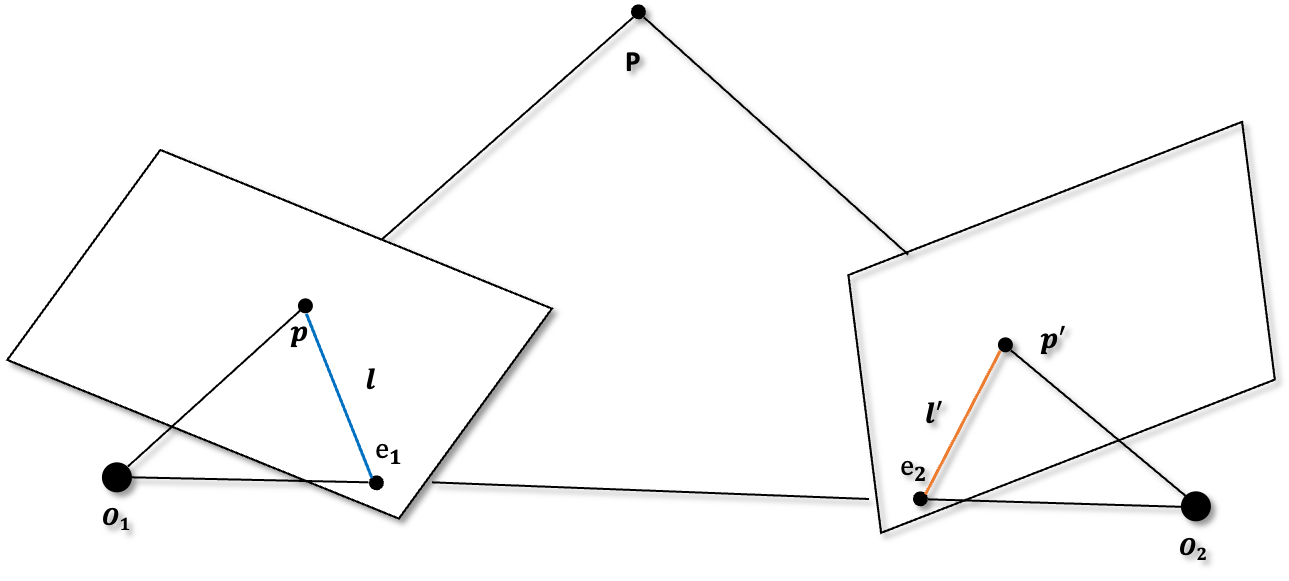
\includegraphics[width=0.8\textwidth]{images/base_matrix.png}
		\end{center}
		\caption{两图像之间的极几何约束,$O_1,O_2$为相机\textbf{光心},$O_1O_2$为\textbf{基线},$p,p^{\prime}$为$P$在两个像素平面的像,$e_1,e_2$为\textbf{极点},$l,l^{\prime}$为\textbf{极线}}
	\end{figure}

	\begin{equation}
		{p^{\prime}}^T \mathbf{F} p = 0 \label{f_constrain}
	\end{equation}

	\begin{align}
		\mathbf{F} = {K^{\prime}}^T [T{_{\times}}] RK^{-1} \label{base_matrix}
	\end{align}

	\begin{equation}
		T_{\times} = \begin{bmatrix}
			&0 \quad &-t_z \quad & t_y\\
			&t_z \quad &0 \quad &-t_x\\
			&-t_y \quad &t_x \quad &0
		\end{bmatrix}
	\end{equation}

	这里有很多概念需要说明,
	\begin{itemize}
		\item 第一个相机坐标系选定为世界坐标系
		\item $K$是第一个相机的内参矩阵
		\item $K^{\prime}$是第二个相机内参矩阵,$R,T$是相对世界坐标系的旋转矩阵和平移向量
		\item $T_{\times}$是由第二个相机的平移向量张成的矩阵,这个矩阵秩为$2$,因此$F$的秩也为$2$
	\end{itemize}

	因为$p^{\prime}$在极线$l^{\prime}$上,所以${{p^{\prime}}^Tl^{\prime} = 0}$,结合(\ref{f_constrain})可知,

	$$
		l^{\prime} = Fp
	$$
	因此,基础矩阵描述了点之间的约束关系,而非一一对应关系,实际上一个点对应到目标平面上的一条极线。\\

	如上图中点$p$的像对应到第二个像素平面的极线$l^{\prime}$上,虽然还找不到具体的对应点,但可以缩小目标点搜索的范围。\\

	能否从(\ref{f_constrain})中分离出$p^{\prime}$的表示呢?显然$p^{\prime}$有无穷多组解,因为极线上所有的点都是对应的解,分离表示方式会在后边提到。

\subsection{单应矩阵}

	如果拍摄场景是一个平面,而非3D物体,基础矩阵会更加简单,称为\textbf{单应矩阵}

	\begin{align}
		H = K^{\prime} \left(R +t \mathbf{n}_d^T\right) K^{-1} \label{homograph_matrix}
	\end{align}

	其中,$\mathbf{n}_d = \mathbf{n}/d$\\

	这里还要说明,
	\begin{itemize}
		\item 世界坐标系为第一个相机坐标系
		\item $\mathbf{n}$为场景平面在世界坐标系中的法向量,$d$为坐标原点到平面的距离
		\item 场景平面的方程为$\mathbf{n}^T \tilde{P} = d$,$\tilde{P}$为欧式坐标
		\item $K,R,t, K^{\prime}$意义同基础矩阵定义
	\end{itemize}

	如此可得到如下对应关系,

	\begin{equation}
		P^{\prime} = HP 
	\end{equation}

	不同于基础矩阵,点对应极线,单应矩阵描述了点之间一一对应关系,这也是“单应”的意义。\\

	单应矩阵$H$变换后的点对$p,p^{\prime}$依然服从基础矩阵的约束(也称$H$与$F$相容),

	$$
		{p^{\prime}}^T F p = 0 \Rightarrow p H^T F p = 0
	$$

	反之,对任意的矩阵$H$,只要满足 $H^TF + HF^T = 0$,则$H$是从某个平面诱导出的与$F$相容的单应矩阵。\\

	一般情况下只知道两个相机相对世界坐标系的旋转和平移$R_1,t_1,R_2, t_2$,并不清楚相对旋转和平移,(\ref{homograph_matrix})中的$R,t$需要求解,很明显,

	\begin{align*}
		R &= R_2R_1^{-1}\\
		t &= t_2 - R_2R_1^{-1}t_1
	\end{align*}

	(\ref{homograph_matrix})可重写为,

	\begin{align}
		H_d &= K_2 \left(R_2R_1^{-1} +\left(t_2 - R_2R_1^{-1}t_1\right) \mathbf{n}_d^T\right) K_1^{-1} \label{new_homograph_matrix}
	\end{align}	

	这个丑陋的式子是单应矩阵的正确版本,原论文中的公式虽然漂亮但是错误的。后面会看到,在实现中根本不需要使用这个式子。

\subsection{$p^{\prime}$分离表示}

	\definition 相机\textbf{内参矩阵}为$K$($3 \times 3$),相机在世界坐标系中的旋转矩阵为$R$($3 \times 3$),平移为$T$($3 \times 1$),$[R\quad T]$为相机\textbf{外参矩阵},$M = K[R\quad T]$为相机\textbf{投影矩阵},是一个$3 \times 4$矩阵。\\

	把相机A(\textbf{ref})像素平面上一个点$x_1$,投影到相机B(\textbf{src})像素平面上的流程为:
	\begin{itemize}
		\item 将$x_1$从\textbf{ref}像素坐标系反投影到世界坐标系得到点$P$
		\item 将$P$投影到\textbf{src}像素坐标系
	\end{itemize}

	将$P$投影到\textbf{ref}像素平面的的过程为,

	$$
		X_1 = K_1[R_1\quad T_1]
		\begin{bmatrix}
			P\\
			1
		\end{bmatrix} = K_1(R_1P + T_1)
	$$

	因此,
	$$
		P = R_1^{-1}\left(K_1^{-1}X_1 - T_1\right)
	$$

	投影到\textbf{src}像素平面的过程为,

	\begin{align}
		X_2 &= K_2[R_2 \quad T_2] 		
		\begin{bmatrix}
			P\\
			1
		\end{bmatrix} \\
		&= K_2[R_2 \quad T_2] 		
		\begin{bmatrix}
			 R_1^{-1}\left(K_1^{-1}X_1 - T_1\right)\\
			1
		\end{bmatrix}\\
		&=\left[
			K_2R_2\left(K_1R_1\right)^{-1} \quad -\left(K_2R_2\right)R_1^{-1}T_1 +K_2T_2
		\right]
		\begin{bmatrix}
			 X_1\\
			1
		\end{bmatrix}\\		
	\end{align}

	投影矩阵为,

	\begin{equation}
		N = \left[
			K_2R_2\left(K_1R_1\right)^{-1} \quad -\left(K_2R_2\right)R_1^{-1}T_1 +K_2T_2 \label{project_matrix}
		\right]	
	\end{equation}

	是一个$3 \times 4$的矩阵,变换对象是\textbf{ref}坐标系的齐次坐标。\\

	这个变换矩阵是否合理呢,我们拿单应矩阵验证一下:\\

	如果以第一个相机坐标系为世界坐标系,场景是一张平面,$N$应该与单应矩阵(\ref{homograph_matrix})一致。\\

	此时,$R_1 = I, T_1 = \mathbf{0}$,

	$$
		N = \left[K_2R_2K_1^{-1} \quad K_2T_2\right]
	$$

	$H$是$3 \times 3$矩阵与$N$维度不一致,所谓一致是指,

	$$
		H\tilde{P} = N
		\begin{bmatrix}
			\tilde{P}\\
			1
		\end{bmatrix} \Rightarrow K_2\left(R_2 + T_2\mathbf{n}_d^T\right)K_1^{-1}\tilde{P} = K_2R_2K_1^{-1}\tilde{P} + K_2T_2
	$$
	
	整理一下,应该存在如下等式,
	$$
		K_2R_2K_1^{-1}\tilde{P} + K_2T_2\mathbf{n}_d^TK_1^{-1}\tilde{P} = K_2R_2K_1^{-1}\tilde{P} + K_2T_2
	$$

	第一项是相同的,只需验证
	$$
		K_2T_2\mathbf{n}_d^TK_1^{-1}\tilde{P} = K_2T_2
	$$

	因为场景是一个平面,根据定义$\mathbf{n}_d^TK_1^{-1}\tilde{P} = 1$,所以此时的$N$的确与单应矩阵一致。所以矩阵$N$蕴含了单应变换,是一种统一表达,

	$$
		p^{\prime} = Np
	$$

	将$p^{\prime}$带入(\ref{f_constrain})中,可验证$p^{\prime},p$满足基础矩阵约束。\\

	$N$的表示看不清变换的本质,也不简洁,下面将相机投影矩阵扩充为一个$4 \times 4$的可逆矩阵,
	$$
		M_i = \begin{bmatrix}
			K_iR_i,&K_iT_i\\
			\mathbf{0}_{1\times 3},& \mathbf{1}_{1\times 1}
		\end{bmatrix}
	$$

	经过计算可知,
	\begin{equation}
		N = M_2M_1^{-1} \label{simply_N}
	\end{equation}

	这个意义非常清楚,将$X_1$通过$M_1^{-1}$反投影到世界坐标系,再通过$M_2$投影到相机B坐标系,并且通过$N$矩阵的一般性,隐藏了单应变换的细节。pytorch版本的实现用的就也是这个公式。\\

	还需要考虑反投影尺度问题,考虑(\ref{inverse_proj}),(\ref{project_matrix})需修改为,
	\begin{equation}
		N_k = \left[
					kK_2R_2\left(K_1R_1\right)^{-1} \quad -\left(K_2R_2\right)R_1^{-1}T_1 +K_2T_2 \label{project_matrix}\right]	
	\end{equation}

	上式表明,尺度$k$只是作用在旋转矩阵上,对平移向量没有影响,在具体实现代码时可将尺度作用在(\ref{simply_N})的旋转矩阵上。

\section{MVSNet}
	MVSNet并没有输入$1200 \times 1600$的图片,而是下采样到$512 \times 640$,过特征提取后,生成$128 \times 160 \times 32$的特征图,其对应的深度图也被处理成$128 \times 160$。\\

	输出为参考图的深度值,GroundTruth也是参考图的深度值,但被下采样到$128 \times 160$。 处理分几个步骤,

	\begin{itemize}
		\item MVSNet每次输入3张图,一张为ref,2张作为src,经过特征提取后,得到三个$128 \times 160 \times 32$的特征图
		
		\item 采用192个深度单位,通过单应变换将ref特征图分别变换到两个src相机姿态下,得到两个$192 \times 128 \times 160 \times 32$的特征图,称为\textbf{Feauture Volume}

		\item ref特征图也通过192个单位进行深度离散,也得到一个\textbf{Feauture Volume},如此总共有3个\textbf{Feauture Volume},其维度为$192 \times 128 \times 160 \times 32$

		\item 计算三个\textbf{Feauture Volume}的方差,结果作为\textbf{Cost Volume};进行3D卷积,通过softmax沿着深度方向作概率归一化,结果又称为\textbf{Probability Volume},维度为$192 \times 128 \times 160$

		\item 沿\textbf{Probability Volume}深度方向计算深度期望值,得到维度为$128 \times 160$的深度特征图,
			$$
				D = \sum_{d = d_{min}}^{d_{max}} d \times \mathbf{P}(d)
			$$

			论文中提到,这一步实际想对\textbf{Probability Volume}作一个$\arg\max$操作,选出当前位置最可能的深度值,但是$\arg\max$无法求导,无法进行梯度回传,所以用这个所谓的soft $\arg\min$机制代替,后面我们会专门讨论

		\item 通过$L_1$回归参考图的深度值;这里只有参考图的深度值为GroundTruth,src图的深度值未使用。
	\end{itemize}
	

	





\bibliography{math}
\end{document}